\chapter{Lec 02 - Graphs Representation and DFS}

\section{Graphs Representation}
How can we encode a graph for using it in an algorithm ? A first simple solution can consist of using a list of vertices $L_{V}$ and a list of edges $L_{E}$. However, this representation does not allow for fast algorithms.\newline\newline
In order to allow for \textbf{direct access to edges}, the following data structures are used in addition to $L_{V}$ and $L_{E}$.
\begin{itemize}
    \item \textbf{Adjacency list:} An array of $n$ list, one for each vertex $v \in V$, each containing all the vertices adjacent to $v$.
    \begin{itemize}
        \item Pro: Space required $\rightarrow \Theta(n + m)$, that is \textbf{linear}.
        
        \item Cons: No quick way to determine if an edge is present in the graph.
    \end{itemize}

    \item \textbf{Adjacency matrix:} A $n \times n$ matrix $A$ such that $A[i,j] = 1$ if $edge(i,j) \in E$, 0 otherwise.\newline\newline
    \textbf{Example:}\newline\newline
    \begin{center}
        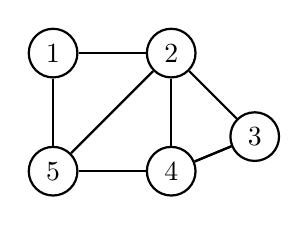
\begin{tikzpicture}[node distance={15mm}, thick, main/.style = {draw, circle}] 
            \node[main] (1) {$1$}; 
            \node[main] (2) [right of=1] {$2$}; 
            \node[main] (3) [below right of=2] {$3$}; 
            \node[main] (4) [below of=2] {$4$}; 
            \node[main] (5) [below of=1] {$5$}; 
            \draw (1) -- (2); 
            \draw (1) -- (5); 
            \draw (2) -- (5);
            \draw (2) -- (4);
            \draw (5) -- (4);
            \draw (3) -- (4); 
            \draw (5) -- (4);
            \draw (4) -- (3);
            \draw (2) -- (3);
        \end{tikzpicture}
    \end{center}
    The Adjacency matrix of the graph above is the following:
    \[\begin{bmatrix}
        0 & 1 & 0 & 0 & 1 \\
        1 & 0 & 1 & 1 & 1 \\
        0 & 1 & 0 & 1 & 0 \\
        0 & 1 & 1 & 0 & 1 \\
        1 & 1 & 0 & 1 & 0
    \end{bmatrix}\]

    In undirected graphs this matrix is \textbf{symmetric}, while in directed graphs it is \textbf{asymmetric}. In case of a weighted graph, each cell of the matrix has either the value of the edge weight $w$ or $-$.
    \begin{itemize}
        \item Pro: Quick to determine if a given edge is present.
        \item Cons: Space required $\rightarrow \Theta(n^{2})$.
    \end{itemize}
\end{itemize}

\section{Graph search and its application}
Graph search algorithms provide a systematic way to \textbf{explore} a graph starting from a vertex $s \in V$ visiting all the vertices.\newline\newline
The most famous algorithms are:
\begin{itemize}
    \item \textbf{Depth-first search} (DFS).
    \item \textbf{Breadth-first search} (BFS).
\end{itemize}
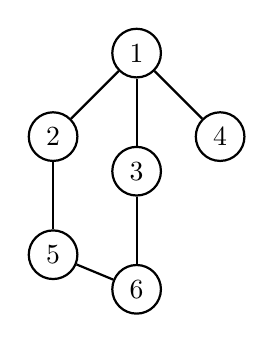
\begin{tikzpicture}[node distance={15mm}, thick, main/.style = {draw, circle}] 
            \node[main] (1) {$1$}; 
            \node[main] (2) [below left of=1] {$2$}; 
            \node[main] (3) [below of=1] {$3$}; 
            \node[main] (4) [below right of=1] {$4$}; 
            \node[main] (5) [below of=2] {$5$};
            \node[main] (6) [below of=3] {$6$};
            \draw (1) -- (2); 
            \draw (1) -- (3); 
            \draw (1) -- (4);
            \draw (2) -- (5);
            \draw (3) -- (6);
            \draw (5) -- (6);
\end{tikzpicture}\newline\newline
\textbf{DFS:} $1 \rightarrow 2 \rightarrow 5 \rightarrow 6 \rightarrow 3 \rightarrow 4$\newline
\textbf{BFS:} $1 \rightarrow 2 \rightarrow 3 \rightarrow 4 \rightarrow 5 \rightarrow 6$

\subsection{DFS Algorithm}
The DFS algorithm is a recursive algorithm that, starting from a source $s \in V$, visits all the vertices of the \textbf{connected component} $C_{s} \subseteq G$ containing $s$.
\begin{itemize}
    \item We use the adjacency list as graph representation.
    \item Every vertex $v$ has a field $L_{v}[v].ID$ which can either be 1 if the vertex has been visited, 0 otherwise.
    \item Every edge $e$ has a field $L_{E}[e].Label$ which can either be null or \textit{Discovery edge / Back edge} \footnote{During the search, we label the edges. This operation is useful for solving some problems.}.
\end{itemize}
Initially, every vertex ID is 0 and each edge Label is null.

\begin{algorithm}
\caption{DFS}\label{dfs}
    \begin{algorithmic}[1]
    \Procedure{DFS (G, v)}{}
    \State $\text{visit } v$
    \State $L_{V}[v].ID \gets 1$
    \For{$e \in G.\text{incidentEdges}(v):$}
        \If{$L_{E}[e].label = null$}
            \State $w \gets G.\text{opposite}(v, e)$
            \If{$L_{V}[w].ID = 0$}
                \State $L_{E}[e].label \gets \textit{Discovery Edge}$
                \State DFS(G, w)
            \Else
                \State $L_{E}[e].label \gets \textit{Back Edge}$
            \EndIf
            
        \EndIf
    \EndFor
    \EndProcedure
    \end{algorithmic}
\end{algorithm}
\textbf{Example:}\newline\newline
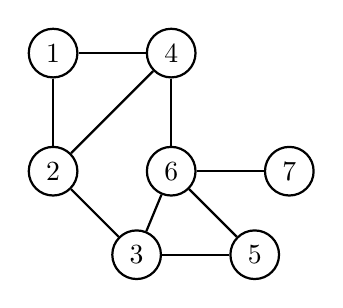
\begin{tikzpicture}[node distance={15mm}, thick, main/.style = {draw, circle}] 
            \node[main] (1) {$1$}; 
            \node[main] (2) [below of=1] {$2$}; 
            \node[main] (3) [below right of=2] {$3$}; 
            \node[main] (4) [right of=1] {$4$}; 
            \node[main] (5) [right of=3] {$5$};
            \node[main] (6) [below of=4] {$6$};
            \node[main] (7) [right of=6] {$7$};
            \draw (1) -- (2); 
            \draw (1) -- (4); 
            \draw (4) -- (2);
            \draw (4) -- (6);
            \draw (2) -- (3);
            \draw (3) -- (6);
            \draw (3) -- (5);
            \draw (5) -- (6);
            \draw (6) -- (7);
\end{tikzpicture}\newline\newline
\textbf{DFS:} $1 \rightarrow 2 \rightarrow 3 \rightarrow 5 \rightarrow 6 \rightarrow 4 \rightarrow 7$\newline\newline
\subsection{Correctness of the algorithm}
At the end of the algorithm:
\begin{enumerate}
    \item All the vertices of $C_{s}$ have been visited, and all the edges in $C_{s}$ are labelled either \textit{Discovery Edge} or \textit{Back Edge}

    \item The set of \textit{Discovery Edges} is a \textbf{spanning tree} $T$ of $C_{s}$.
\end{enumerate}
\textbf{Proof:}
\begin{enumerate}
    \item A vertex $u$ is visited when DFS($G, u$) is called. Assume by contradiction that $\exists u \in C_{s}$ not visited. Since $C_{s}$ is connected, it exists a path from $s$ to $u$ $s=u_{0} \rightarrow u_{1} \rightarrow u_{2}, ..., u_{k}=u$. Let $u_{i}$ be the first unvisited vertex in the path. When DFS is called on $u_{i - 1}$ it finds $u_{i}$ not visited and therefore DFS($G, u_{i}$) is called. Then $u_{i}$ is visited. This is in contradiction with the initial hypothesis.\newline\newline
    DFS is called $\forall v \in C_{s}$. Therefore, all incident edges on $v$ are labelled, by construction.

    \item DFS is called for every vertex $v \in C_{s}$ once, and $\forall v \neq s$ it exists a vertex $u$ such that the edge $(u, v)$ exists and is labelled \textit{Discovery Edge}. This implies that $\forall v \in C_{s} \,\, v \neq s$ it exists a \textit{father} and going back father to father, eventually $s$ is reached. Then, the set of \textit{Discovery Edges} is a rooted tree that \textit{touches} all the vertices of $C_{s}$, that is, a spanning tree of $C_{s}$.
\end{enumerate}

\subsection{Complexity of the algorithm}
Given:
\begin{itemize}
    \item $n_{s}$: number of vertices of $C_{s}$.
    \item $m_{s}$: number of edges of $C_{s}$.
\end{itemize}
The complexity of DFS is:
\[\Theta\left( \sum_{v \in C_{s}} d(v)\right) = \Theta(m_{s})\]
Note that $C_{s}$ is connected, so $m_{s} \geq n_{s} - 1 \rightarrow m_{s} = \Omega(n_{s})$.

\vspace{50pt}
\subsection{DFS Extension}
DFS($G, s$) visits only the connected component of $s$. If the graph is not connected and we want to visit all the graph, the DFS algorithm can be extended as follows:
\begin{algorithm}
\caption{DFS}\label{dfs_2}
    \begin{algorithmic}[1]
    \Procedure{DFS ($G, v$)}{}
        \For{$v \gets 1 \,\, \text{to } n$}
            \If{$L_{V}[v].ID = 0$}
                \State DFS($G, v$)
            \EndIf
        \EndFor
    \EndProcedure
    \end{algorithmic}
\end{algorithm}\newline\newline
Its complexity is $\Theta(n + m)$ because it scans over all the vertices.

\subsection{Problem 1}
Given a graph $G$ and two vertices $s, t$, determines, if exists, a path from $s$ to $v$.\newline\newline
Modified version of DFS:
\begin{algorithm}
\caption{DFS}\label{modified_dfs}
    \begin{algorithmic}[1]
    \Procedure{DFS (G, v)}{}
    \State $\text{visit } v$
    \State $L_{V}[v].ID \gets 1$
    \For{$e \in G.\text{incidentEdges}(v):$}
        \If{$L_{E}[e].label = null$}
            \State $w \gets G.\text{opposite}(v, e)$
            \If{$L_{V}[w].ID = 0$}
                \State $L_{E}[e].label \gets \textit{Discovery Edge}$
                \State $L_{V}[w].parent \gets v$
                \State DFS(G, w)
            \Else
                \State $L_{E}[e].label \gets \textit{Back Edge}$
            \EndIf
            
        \EndIf
    \EndFor
    \EndProcedure
    \end{algorithmic}
\end{algorithm}
\begin{itemize}
    \item $\forall v \in V$ add a field $L_{V}[v].parent$
    \item Modify the DFS algorithm such that when a \textit{Discovery Edge} $(v,w)$ is labelled, we set $L_{V}[w].parent = v$.
    \item Run DFS($G, s$), starting from the source $s$, and check if $t$ jas been visited. If $t$ has not been visited, there is no path from $s$ to $t$, otherwise build the path starting from $t$ and going backward parent to parent until $s$ is reached.
\end{itemize}
The complexity of the algorithm is the same as DFS since we only added constant operations.

\vspace{50pt}
\subsection{Problem 2}
Given a graph determine a cycle (if any):
\begin{algorithm}
\caption{DFS}\label{modified_dff_cycles}
    \begin{algorithmic}[1]
    \Procedure{DFS (G, v)}{}
    \State $\text{visit } v$
    \State $L_{V}[v].ID \gets 1$
    \For{$e \in G.\text{incidentEdges}(v):$}
        \If{$L_{E}[e].label = null$}
            \State $w \gets G.\text{opposite}(v, e)$
            \If{$L_{V}[w].ID = 0$}
                \State $L_{E}[e].label \gets \textit{Discovery Edge}$
                \State $L_{V}[w].parent \gets v$
                \State DFS(G, w)
            \Else
                \State $L_{E}[e].label \gets \textit{Back Edge}$
                \State $L_{E}[e].ancestor \gets w$
            \EndIf
        \EndIf
    \EndFor
    \EndProcedure
    \end{algorithmic}
\end{algorithm}
\begin{itemize}
    \item $\forall v \in V$ add a field $L_{V}[v].parent$
    \item $\forall e \in E$ add a field $L_{E}[e].ancestor$
    \item Modify the DFS algorithm such that if a \textit{Discovery Edge} $(v,w)$ is labelled we set $L_{V}[w].parent = v$, and if $(v,w)$ is labelled as \textit{Back Edge}, we set $L_{E}[e].ancestor = w$.
    \item Run DFS on each connected component.
    \item Check all the edges. When a \textit{Back Edge} $e = (v, w)$ is found and $L_{E}[e].ancestor = w$, return a cycle adding to $e$ all the edges found in the path from $v$ to $w$. 
\end{itemize}
Since we run DFS on each connected component, the complexity is $\Theta(n + m)$ (we scan all the nodes).

